\documentclass[12pt,letterpaper]{hmcpset}
\usepackage[margin=1in]{geometry}
\usepackage{graphicx}

% info for header block in upper right hand corner
\name{ }
\class{Math 60}
\assignment{HW 9}
\duedate{Friday, May 27, 2016}

\newcommand{\pn}[1]{\left(#1\right)}
\newcommand{\abs}[1]{\left|#1\right|}
\newcommand{\bk}[1]{\left[#1\right]}
\newcommand{\cbk}[1]{\left\{#1\right\}}
\newcommand{\s}[1]{\sqrt{#1}}
\newcommand{\f}[2]{\frac{#1}{#2}}
\renewcommand{\labelenumi}{{(\alph{enumi})}}

\begin{document}

\problemlist{5.5.\{9, 20, 25, 31, 34, 38\}}

\begin{problem}[Colley 5.5.9]
    Evaluate the integral
    \[
        \int_0^2\int_{x/2}^{(x/2)+1}x^5(2y-x)e^{(2y-x)^2}~dy~dx
    \]
    by making the substitution $u=x$, $v=2y-x$.
\end{problem}
\begin{solution}
    \vfill
\end{solution}
\newpage

\begin{problem}[Colley 5.5.20]
    Find the total area enclosed inside the rose $r=\sin
    2\theta$. (Hint: Sketch the curve and find the area inside a
    single leaf.)
\end{problem}
\begin{solution}
    \vfill
\end{solution}
\newpage

\begin{problem}[Colley 5.5.25]
    Evaluate
    \[
        \iint_D\cos(x^2+y^2)~dA,
    \]
    where $D$ is the shaded region in Figure 5.106.
    \begin{center}
        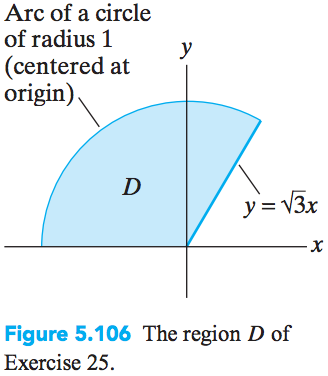
\includegraphics{img/5_5_25}
    \end{center}
\end{problem}
\begin{solution}
    \vfill
\end{solution}
\newpage

\begin{problem}[Colley 5.5.31]
    Determine
    \[
        \iiint_W(x^2+y^2+2z^2)~dV,
    \]
    where $W$ is the solid cylinder defined by the inequalities
    $x^2+y^2\leq4$, $-1\leq z\leq2$.
\end{problem}
\begin{solution}
    \vfill
\end{solution}
\newpage

\begin{problem}[Colley 5.5.34]
    In Exercises 34 and 35, determine the values of the given
    integrals, where $W$ is the region bounded by the two spheres
    $x^2+y^2+z^2=a^2$ and $x^2+y^2+z^2=b^2$, for $0<a<b$.
    \[
        \iiint_W\f{dV}{\s{x^2+y^2+z^2}}
    \]
\end{problem}
\begin{solution}
    \vfill
\end{solution}
\newpage

\begin{problem}[Colley 5.5.38]
    Determine
    \[
        \iiint_W\pn{2+\s{x^2+y^2}}~dV,
    \]
    where $W=\cbk{(x,y,z)|\s{x^2+y^2}\leq z/2\leq3}$.
\end{problem}
\begin{solution}
    \vfill
\end{solution}
\end{document}
